% -*- coding: utf-8 -*-
%-------------------------designed by zcf--------------
\documentclass[UTF8,a4paper,10pt]{ctexart}
\usepackage[left=3.17cm, right=3.17cm, top=2.74cm, bottom=2.74cm]{geometry}
\usepackage{amsmath}
\usepackage{graphicx,subfig}
\usepackage{float}
\usepackage{cite}
\usepackage{caption}
\usepackage{enumerate}
\usepackage{booktabs} %表格
\usepackage{multirow}
\newcommand{\tabincell}[2]{\begin{tabular}{@{}#1@{}}#2\end{tabular}}  %表格强制换行
%-------------------------字体设置--------------
\usepackage{times} 
\newcommand{\yihao}{\fontsize{26pt}{36pt}\selectfont}           % 一号, 1.4 倍行距
\newcommand{\erhao}{\fontsize{22pt}{28pt}\selectfont}          % 二号, 1.25倍行距
\newcommand{\xiaoer}{\fontsize{18pt}{18pt}\selectfont}          % 小二, 单倍行距
\newcommand{\sanhao}{\fontsize{16pt}{24pt}\selectfont}  %三号字
\newcommand{\xiaosan}{\fontsize{15pt}{22pt}\selectfont}        % 小三, 1.5倍行距
\newcommand{\sihao}{\fontsize{14pt}{21pt}\selectfont}            % 四号, 1.5 倍行距
\newcommand{\banxiaosi}{\fontsize{13pt}{19.5pt}\selectfont}    % 半小四, 1.5倍行距
\newcommand{\xiaosi}{\fontsize{12pt}{18pt}\selectfont}            % 小四, 1.5倍行距
\newcommand{\dawuhao}{\fontsize{11pt}{11pt}\selectfont}       % 大五号, 单倍行距
\newcommand{\wuhao}{\fontsize{10.5pt}{15.75pt}\selectfont}    % 五号, 单倍行距
%-------------------------章节名----------------
\usepackage{ctexcap} 
\CTEXsetup[name={,、},number={ \chinese{section}}]{section}
\CTEXsetup[name={(,)},number={\chinese{subsection}}]{subsection}
\CTEXsetup[name={,.},number={\arabic{subsubsection}}]{subsubsection}
%-------------------------页眉页脚--------------
\usepackage{fancyhdr}
\pagestyle{fancy}
\lhead{\kaishu \leftmark}
% \chead{}
\rhead{\kaishu 计算机系统设计作业报告}%加粗\bfseries 
\lfoot{}
\cfoot{\thepage}
\rfoot{}
\renewcommand{\headrulewidth}{0.1pt}  
\renewcommand{\footrulewidth}{0pt}%去掉横线
\newcommand{\HRule}{\rule{\linewidth}{0.5mm}}%标题横线
\newcommand{\HRulegrossa}{\rule{\linewidth}{1.2mm}}
%-----------------------伪代码------------------
\usepackage{algorithm}  
\usepackage{algorithmicx}  
\usepackage{algpseudocode}  
\floatname{algorithm}{Algorithm}  
\renewcommand{\algorithmicrequire}{\textbf{Input:}}  
\renewcommand{\algorithmicensure}{\textbf{Output:}} 
\usepackage{lipsum}  
\makeatletter
\newenvironment{breakablealgorithm}
  {% \begin{breakablealgorithm}
  \begin{center}
     \refstepcounter{algorithm}% New algorithm
     \hrule height.8pt depth0pt \kern2pt% \@fs@pre for \@fs@ruled
     \renewcommand{\caption}[2][\relax]{% Make a new \caption
      {\raggedright\textbf{\ALG@name~\thealgorithm} ##2\par}%
      \ifx\relax##1\relax % #1 is \relax
         \addcontentsline{loa}{algorithm}{\protect\numberline{\thealgorithm}##2}%
      \else % #1 is not \relax
         \addcontentsline{loa}{algorithm}{\protect\numberline{\thealgorithm}##1}%
      \fi
      \kern2pt\hrule\kern2pt
     }
  }{% \end{breakablealgorithm}
     \kern2pt\hrule\relax% \@fs@post for \@fs@ruled
  \end{center}
  }
\makeatother
%------------------------代码-------------------
\usepackage{xcolor} 
\usepackage{listings} 
\usepackage{fontspec}
\newfontfamily\menlo{Menlo}
\setmonofont[Mapping={}]{Monaco} 
\definecolor{mygreen}{rgb}{0,0.6,0}
\definecolor{mygray}{rgb}{0.5,0.5,0.5}
\definecolor{mymauve}{rgb}{0.58,0,0.82}
\lstset{ %
backgroundcolor=\color{white},   % choose the background color
basicstyle=\footnotesize\ttfamily,        % size of fonts used for the code
columns=fullflexible,
breaklines=true,                 % automatic line breaking only at whitespace
captionpos=b,                    % sets the caption-position to bottom
tabsize=4,
commentstyle=\color{mygreen},    % comment style
escapeinside={\%*}{*)},          % if you want to add LaTeX within your code
keywordstyle=\color{blue},       % keyword style
stringstyle=\color{mymauve}\ttfamily,     % string literal style
frame=single,
rulesepcolor=\color{red!20!green!20!blue!20},
numbers=left,
 numberstyle=\tiny\menlo
% identifierstyle=\color{red},
% language=c++,
}
%------------超链接----------
\usepackage[colorlinks,linkcolor=black,anchorcolor=blue]{hyperref}
%------------------------TODO-------------------
\usepackage{enumitem,amssymb}
\newlist{todolist}{itemize}{2}
\setlist[todolist]{label=$\square$}
% for check symbol 
\usepackage{pifont}
\newcommand{\cmark}{\ding{51}}%
\newcommand{\xmark}{\ding{55}}%
\newcommand{\done}{\rlap{$\square$}{\raisebox{2pt}{\large\hspace{1pt}\cmark}}\hspace{-2.5pt}}
\newcommand{\wontfix}{\rlap{$\square$}{\large\hspace{1pt}\xmark}}
%------------------------水印-------------------
\usepackage{tikz}
\usepackage{xcolor}
\usepackage{eso-pic}

\newcommand{\watermark}[3]{\AddToShipoutPictureBG{
\parbox[b][\paperheight]{\paperwidth}{
\vfill%
\centering%
\tikz[remember picture, overlay]%
  \node [rotate = #1, scale = #2] at (current page.center)%
    {\textcolor{gray!80!cyan!30!magenta!30}{#3}};
\vfill}}}



%———————————————————————————————————————————正文———————————————————————————————————————————————
%----------------------------------------------
\begin{document}
\begin{titlepage}
    \begin{center}
    
\includegraphics[width=0.8\textwidth]{NKU.png}\\[1cm]    
    \textsc{\Huge \kaishu{\textbf{南\ \ \ \ \ \ 开\ \ \ \ \ \ 大\ \ \ \ \ \ 学}} }\\[0.9cm]
    \textsc{\huge \kaishu{\textbf{计\ \ 算\ \ 机\ \ 学\ \ 院}}}\\[0.5cm]
    \textsc{\Large \textbf{计算机系统设计作业报告}}\\[0.8cm]
    \HRule \\[0.9cm]
    { \LARGE \bfseries PA实验一报告}\\[0.4cm]
    \HRule \\[2.0cm]
    \centering
    \textsc{\LARGE \kaishu{朱浩泽\ 1911530}}\\[0.5cm]
    \textsc{\LARGE \kaishu{年级\ :\ 2019级}}\\[0.5cm]
    \textsc{\LARGE \kaishu{专业\ :\ 计算机科学与技术}}\\[0.5cm]
    \textsc{\LARGE \kaishu{指导教师\ :\ 卢冶}}\\[0.5cm]
    \vfill
    {\Large \today}
    \end{center}
\end{titlepage}
% -------------摘------要--------------
\newpage
% \thispagestyle{empty}
% \renewcommand{\abstractname}{\kaishu \sihao \textbf{摘要}}
%     \begin{abstract}

%         \noindent  %顶格
%         \textbf{\\\ 关键字:Parallel}\textbf{} \\\ \\\
%     \end{abstract}
% % ----------------------------------------------------------------
\tableofcontents
% ----------------------------------------------------------------
\newpage
\watermark{60}{10}{NKU}
\setcounter{page}{1}
\section{概述}
%——————————————————————————————————————
\subsection{实验目的}
熟悉基础设施的各种工具和手段;熟悉寄存器间的存储关系;学习实现简易调试器
补充指令;学习表达式求值,监视点的实现方法
\subsection{实验内容}
\begin{itemize}
  \item \textbf{阶段一}
  \begin{itemize}
    \item [$\circ $] 实现正确的寄存器结构体
    \item [$\circ $] 实现解析命令
    \item [$\circ $] 实现单步执行
    \item [$\circ $] 实现打印寄存器
    \item [$\circ $] 实现内存扫描
  \end{itemize}
  \item \textbf{阶段二}
  \begin{itemize}
    \item [$\circ $] 实现词法分析
    \item [$\circ $] 实现递归求值
    \item [$\circ $] 实现调试中的表达式求值
  \end{itemize}
  \item \textbf{阶段三}
  \begin{itemize}
    \item [$\circ $] 实现断点
    \item [$\circ $] 实现监视点
  \end{itemize}
\end{itemize}
%——————————————————————————————————————
\section{阶段一}
\subsection{实现正确的寄存器结构体}
\begin{itemize}
  \item 为了实现32位、16位、8位寄存器各8个和一个程序计数器eip,我们利用匿名Union各个变量互斥并共享同一内存首地址这一特点,来实现这一结构体
  \item 修改nemu/include/cpu/reg.h中的代码如下
  \begin{lstlisting}[language = C]    
typedef struct {
  union{
    /* data */
    union {
      uint32_t _32;
      uint16_t _16;
      uint8_t _8[2];
    } gpr[8];
    struct 
    {
      rtlreg_t eax, ecx, edx, ebx, esp, ebp, esi, edi;
    };
  };
  vaddr_t eip;
} CPU_state;
  \end{lstlisting}
  \item 在上面的代码中,grp中的的\_32代表的是eax中的32位,\_16代表的是ax中的16位,\_8[2]分别代表的是ah中的8到16位和al中的0到8位
\end{itemize}
\subsection{实现解析命令}
\begin{itemize}
  \item 在nemu/src/monitor/debug/ui.c中实现命令表,其代码如下
  \begin{lstlisting}[language = C]
static struct {
  char *name;
  char *description;
  int (*handler) (char *);
} cmd_table [] = {
  { "help", "Display informations about all supported commands", cmd_help },
  { "c", "Continue the execution of the program", cmd_c },
  { "q", "Exit NEMU", cmd_q },

  /* TODO: Add more commands */

  { "si", "args:[N]; exectue [N] instructions step by step", cmd_si}, //让程序单步执行 N 条指令后暂停执行, 当N没有给出时, 缺省为1
  { "info", "args:r/w;print information about register or watch point ", cmd_info}, //打印寄存器状态
  { "x", "x [N] [EXPR];sacn the memory", cmd_x }, //内存扫描
  { "p", "expr", cmd_p}, //表达式
  { "w", "set the watchpoint", cmd_w}, //添加监视点
  { "d", "delete the watchpoint", cmd_d} //删除监视点
};
  \end{lstlisting}
  \item 其执行效果如下图所示
  \begin{center}
    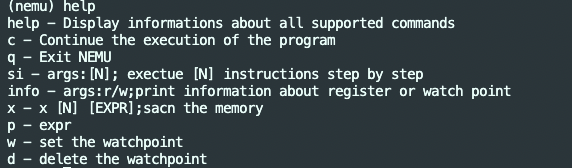
\includegraphics[scale = 0.6]{4}
  \end{center}
  
\end{itemize}
\subsection{实现单步执行}
\begin{itemize}
  \item  在nemu/src/monitor/debug/ui.c添加cmd\_si函数,其代码如下
  \begin{lstlisting}[language = C]
static int cmd_si(char *args) {
  uint64_t N = 0;
  if(args == NULL) {
    N = 1;
  }
  else {
    int temp = sscanf(args, "%lu", &N);
    if(temp <= 0) {
      printf("args error in cmd_si\n");
      return 0;
    }
  }
  cpu_exec(N);
  return 0;
}
  \end{lstlisting}
  \item 执行效果如下图所示,输入si和要执行的步骤N,进行打印
  \begin{center}
    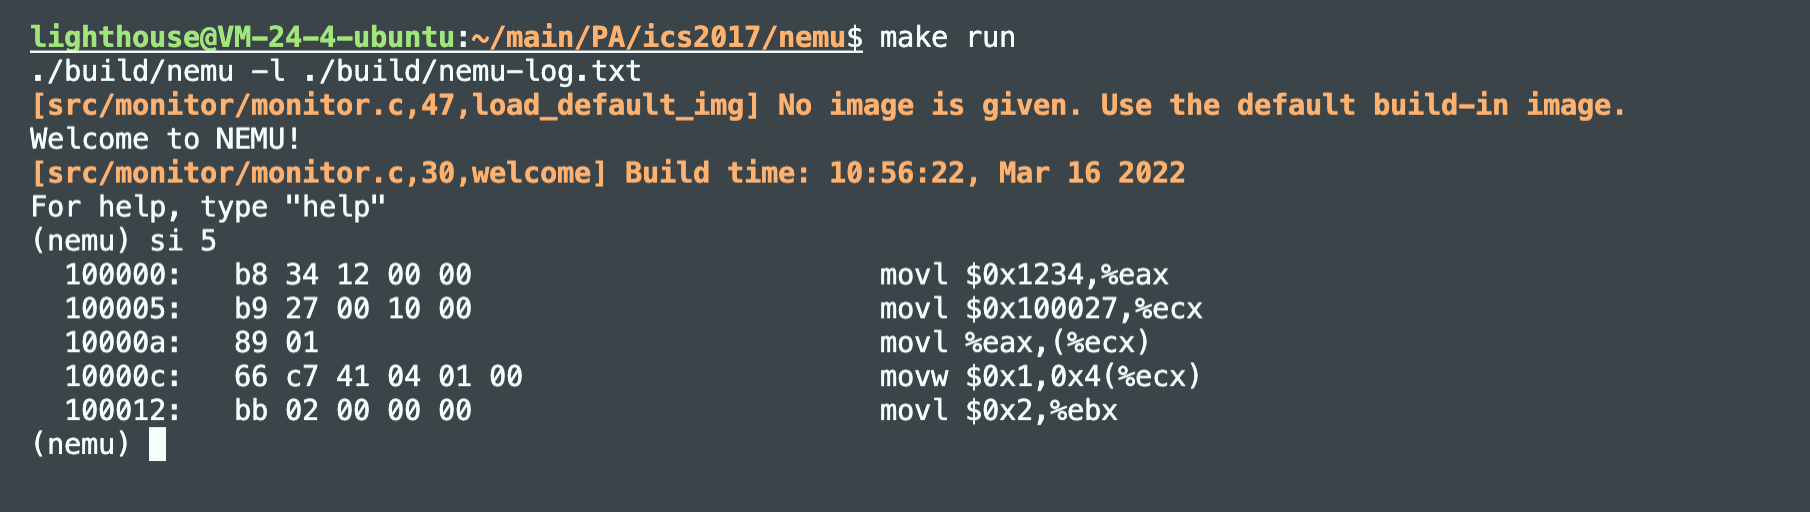
\includegraphics[scale = 0.43]{5}
  \end{center}
\end{itemize}
\subsection{实现打印寄存器}
\begin{itemize}
  \item 在nemu/src/monitor/debug/ui.c添加cmd\_info函数,其代码如下,输入参数r对寄存器直接进行打印,输入参数w对监视点进行打印
  \begin{lstlisting}[language = c++]
static int cmd_info(char *args) {
  char s;
  if(args == NULL) {
    printf("args error in cmd_info (miss args)\n");
    return 0;
  }
  int temp = sscanf(args, "%c", &s);
  if(temp <= 0) {
    //解析失败
    printf("args error in cmd_info\n");
    return 0;
  }
  if(s == 'w') {
    //打印监视点信息
    print_wp();;
    return 0;
  }
  if(s == 'r') {
    //打印寄存器
    //32bit
    for(int i = 0; i < 8; i++) {
      printf("%s  0x%x\n", regsl[i], reg_l(i));
    }
    printf("eip  0x%x\n", cpu.eip);
    //16bit
    for(int i = 0; i < 8; i++) {
      printf("%s  0x%x\n", regsw[i], reg_w(i));
    }
    //8bit
    for(int i = 0; i < 8; i++)
    {
      printf("%s  0x%x\n", regsb[i], reg_b(i));
    }
    return 0;
  }
  //如果产生错误
  printf("args error in cmd_info\n");
  return 0;
}
  \end{lstlisting}
  \item 执行效果如下图所示
  \begin{center}
    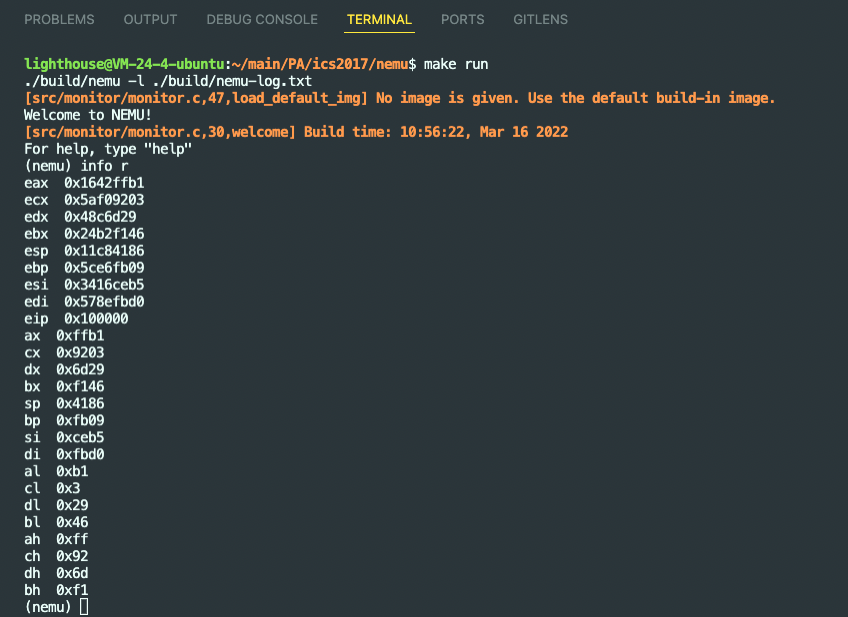
\includegraphics[scale = 0.4]{2}
  \end{center}
\end{itemize}
\subsection{实现内存扫描}
\begin{itemize}
  \item 在nemu/src/monitor/debug/ui.c添加cmd\_x函数,其代码如下
  \begin{lstlisting}[language = C]
static int cmd_x(char *args) {
  int nLen = 0;
  vaddr_t addr;
  int temp = sscanf(args, "%d 0x%x", &nLen, &addr);
  if(temp <= 0) {
    //解析失败
    printf("args error in cmd_si\n");
    return 0;
  }
  printf("Memory:");
  for(int i = 0; i < nLen; i++) {
    if(i % 4 == 0) {
      printf("\n0x%x:  0x%02x", addr + i, vaddr_read(addr + i, 1));
    }  
    else {
      printf("  0x%02x", vaddr_read(addr + i, 1));
    }
  }
  printf("\n");
  return 0;
}
  \end{lstlisting}
  \item 该函数主要是调用了nemu/src/memory/memory.c中的vaddr\_read函数进行内存扫描
  \item 执行效果如下图所示
  \begin{center}
    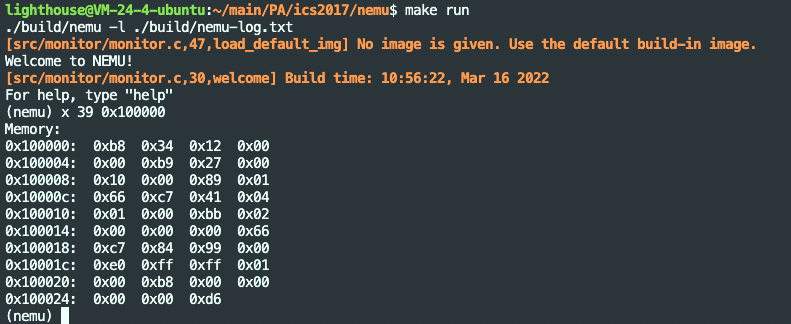
\includegraphics[scale = 0.45]{3}
  \end{center}
\end{itemize}

\section{阶段二}
在本次实验中,要求实现包括+ - * / == != >= <= > < \&\& || ! 指针和正负运算等多种运算,以及十进制数、八进制数、十六进制数等运算。 
\par 在有了编译原理课程的基础后,我们可以知道,表达式求值的过程是先将整个句子切分为各个token,然后对各个token按照赋予的优先级进行分割后求返回值,最终通过这种递归运算求出整个表达式的值。
\par 在这个求值过程中,我们需要注意寄存器的值是可以当作操作数进行运算的,且对于括号的操作跟编译原理中直接利用lex工具,本次实验中需要手写函数进行动态判定,这本质上是一个脱括号的过程,需要判断脱括号后其匹配是否合法。
\par 本节实验主要代码在nemu/src/monitor/debug/exp.c文件中实现
\subsection{词法分析}
\begin{itemize}
  \item 首先我们定义tokens类型和正则表达式来识别tokens,其代码如下
  \begin{lstlisting}[language = C]
enum {
  TK_NOTYPE = 256, 
  TK_NUMBER,
  TK_HEX,
  TK_REG,
  TK_EQ,
  TK_NEQ,
  TK_AND,
  TK_OR,
  TK_NEGATIVE,
  TK_DEREF,
};

static struct rule {
  char *regex;
  int token_type;
} rules[] = {

  /* TODO: Add more rules.
   * Pay attention to the precedence level of different rules.
   */

  {" +", TK_NOTYPE},    // spaces
  {"0x[0-9A-Fa-f][0-9A-Fa-f]*", TK_HEX},
  {"0|[1-9][0-9]*", TK_NUMBER}, //数字
  {"\\$(eax|ecx|edx|ebx|esp|ebp|esi|edi|eip|ax|cx|dx|bx|sp|bp|si|di|al|cl|dl|bl|ah|ch|dh|bh)", TK_REG},
  {"==", TK_EQ},
  {"!=", TK_NEQ},
  {"&&", TK_AND},
  {"\\|\\|", TK_OR},
  {"!", '!'},
  {"\\+", '+'},         
  {"-", '-'},
  {"\\*", '*'},
  {"\\/", '/'},
  {"\\(", '('},
  {"\\)", ')'},
};
  \end{lstlisting}
  \item 修改代码框架中的make\_token函数,对各种类型的输入进行处理,其中八进制数和十六进制数将会被提前处理,而寄存器则将会跳过开头的美元符号,其代码如下
  
  \begin{lstlisting}[language = C]
static bool make_token(char *e) {
int position = 0;
int i;
regmatch_t pmatch;

nr_token = 0;

while (e[position] != '\0') {
  /* Try all rules one by one. */
  for (i = 0; i < NR_REGEX; i ++) {
    if (regexec(&re[i], e + position, 1, &pmatch, 0) == 0 && pmatch.rm_so == 0) {
      char *substr_start = e + position;
      int substr_len = pmatch.rm_eo;

      Log("match rules[%d] = \"%s\" at position %d with len %d: %.*s",
          i, rules[i].regex, position, substr_len, substr_len, substr_start);
      position += substr_len;

      /* TODO: Now a new token is recognized with rules[i]. Add codes
        * to record the token in the array `tokens'. For certain types
        * of tokens, some extra actions should be performed.
        */
      if(substr_len > 32) {
        assert(0);
      }
      if(rules[i].token_type == TK_NOTYPE) {
        break;
      }
      else {
        tokens[nr_token].type = rules[i].token_type;
        switch (rules[i].token_type) {
        case TK_NUMBER:
          strncpy(tokens[nr_token].str, substr_start, substr_len);
          *(tokens[nr_token].str + substr_len) = '\0';
          break;
        case TK_HEX:
          strncpy(tokens[nr_token].str, substr_start + 2, substr_len - 2); //跳过开头的0x
          *(tokens[nr_token].str + substr_len - 2) = '\0';
          break;
        case TK_REG: 
          strncpy(tokens[nr_token].str, substr_start + 1, substr_len - 1); //跳过开头的$
          *(tokens[nr_token].str + substr_len - 1) = '\0';
        }
        printf("Success record : nr_token = %d, dtype = %d, str = %s\n", nr_token, tokens[nr_token].type, tokens[nr_token].str);
        nr_token += 1;
        break;
      }
    }
    if (i == NR_REGEX) {
      return false;
    }
  }

  return true;
}
  \end{lstlisting}
\end{itemize}
\subsection{递归求值}
\begin{itemize}
  \item 首先我们要进行的工作是检查括号匹配,其主要想法是利用一个计数器来计算匹配的数目,如果最终计数器的值不为0则说明括号不匹配,则表达式出错。其代码如下
  \begin{lstlisting}[language = C]
//判断括号的匹配
bool check_parentheses(int p, int q) {
  if(p >= q) {
    //右括号少于左括号
    printf("error:p>=q in check_parntheses\n");
    return false;
  }
  if(tokens[p].type != '(' || tokens[q].type != ')'){
    //括号不匹配
    return false;
  }
  int cnt = 0; //记录当前未匹配的左括号的数目
  for(int curr = p + 1; curr < q; curr++) {
    if(tokens[curr].type == '(') {
      cnt++;
    }
    if(tokens[curr].type == ')') {
      if(cnt != 0) {
        cnt--;
      }
      else {
        //左右括号不匹配
        return false;
      }
    }
  }
  if(cnt == 0) {
    return true;
  }
  else {
    return false;
  }
} 
  \end{lstlisting}
  \item 利用一个函数来计算表达式优先级最低的运算符的位置,如果有同为最低优先级的预算符,返回最后被结合的运算符的索引位置,其代码如下
  \begin{lstlisting}[language = C]
int findDominantOp(int p, int q) {
  int level=0;
  int pos[5]={-1, -1, -1, -1, -1};
  for(int i = p; i < q; i++){
    if(level == 0) {
      if(tokens[i].type == TK_AND || tokens[i].type == TK_OR) {
        pos[0] = i;
      }
      if(tokens[i].type == TK_EQ || tokens[i].type == TK_NEQ) {
        pos[1] = i;
      }
      if(tokens[i].type == '+' || tokens[i].type == '-') {
        pos[2] = i;
      }
      if(tokens[i].type == '*' || tokens[i].type == '/') {
        pos[3] = i;
      }
      if(tokens[i].type == TK_NEGATIVE || tokens[i].type == TK_DEREF || tokens[i].type == '!') {
        pos[4] = i;
      }
    }
    if(tokens[i].type=='(') {
      level++;
    }
    if(tokens[i].type==')') {
      level--;
    }
  }
  for(int i = 0; i < 5; i++) {
    if(pos[i] != -1) {
      return pos[i];
    }
  }
  printf("error in findDominantOp\n");
  printf("[p=%d,q=%d]\n",p,q);
  assert(0);
}
  \end{lstlisting}
  \item 根据实验指导书编写eval函数,用于值的计算,其中的参数p和q分别代表这个子表达式的开始位置和结束为止,其代码如下
  \begin{lstlisting}[language = C]
uint32_t eval(int p, int q) {
  if(p > q) {
    printf("error:p>q in eval, p = %d, q = %d\n", p, q);
    assert(0);
  }
  if(p == q) {
    int num;
    switch (tokens[p].type){
      case TK_NUMBER:
        sscanf(tokens[p].str, "%d", &num);
        return num;
      case TK_HEX:
        sscanf(tokens[p].str, "%x", &num);
        return num;
      case TK_REG: 
        for(int i = 0; i < 8; i++) {
          if(strcmp(tokens[p].str, regsl[i]) == 0) {
            return reg_l(i);
          }
          if(strcmp(tokens[p].str, regsw[i]) == 0) {
            return reg_w(i);
          }
          if(strcmp(tokens[p].str, regsb[i]) == 0) {
            return reg_b(i);
          }
        }
        if(strcmp(tokens[p].str, "eip") == 0) {
          return cpu.eip;
        }
        else {
          printf("error in TK_REG in eval()\n");
          assert(0);
        } 
    }
  }
  if(check_parentheses(p, q) == true) {
    return eval(p + 1, q - 1);
  }
  else {
    int op = findDominantOp(p, q);
    vaddr_t addr;
    int result;
    switch (tokens[op].type) {
      case TK_NEGATIVE: //负号
        return -eval(p + 1, q);
      case TK_DEREF: //指针求值
        addr = eval(p + 1, q);
        result = vaddr_read(addr, 4);
        printf("adddr=%u(0x%x)---->value=%d(0x%08x)\n", addr, addr, result, result);
        return result;
      case '!': 
        result = eval(p + 1, q);
        if(result != 0) {
          return 0;
        }
        else {
          return 1;
        }
    }
    uint32_t val1 = eval(p, op - 1);
    uint32_t val2 = eval(op + 1, q);
    switch(tokens[op].type) {
      case '+':
        return val1 + val2;
      case '-': 
        return val1 - val2;
      case '/':
        return val1 / val2;
      case '*':
        return val1 * val2;
      case TK_EQ:
        return val1 == val2;
      case TK_NEQ: 
        return val1 != val2;
      case TK_AND: 
        return val1 && val2;
      case TK_OR: 
        return val1 || val2;
      default:
        assert(0);
    }
  }
  return 1;
}
  \end{lstlisting}
\end{itemize}
\subsection{实现调试中的表达式求值}
\begin{itemize}
  \item 修改框架代码中的expr函数进行表达式求值的工作,其中主要分为两步:先调用make\_token进行词法分析,再调用eval函数进行求值操作。为了实现这一功能,我们要对token进行有选择保存信息:对于寄存器和数字,我们保存其类型,并利用字符串保存寄存器的名字和数值;对于一般运算符保存token类型;对于加减法需要区分是单目运算符还是双目运算符,其代码如下
  \begin{lstlisting}[language = c]
uint32_t expr(char *e, bool *success) {
  if (!make_token(e)) {
    *success = false;
    return 0;
  }
  /* TODO: Insert codes to evaluate the expression. */
  // TODO();

  // return 0;
  if(tokens[0].type == '-') {
    tokens[0].type = TK_NEGATIVE;
  }
  if(tokens[0].type == '*') {
    tokens[0].type = TK_DEREF;
  }
  for(int i = 1; i < nr_token; i++) {
    if(tokens[i].type == '-') {
      if(tokens[i - 1].type != TK_NUMBER && tokens[i - 1].type != ')') {
        tokens[i].type = TK_NEGATIVE;
      }
    }
    if(tokens[i].type == '*') {
      if(tokens[i - 1].type != TK_NUMBER && tokens[i - 1].type != ')') {
        tokens[i].type = TK_DEREF;
      }
    }
  }
  *success = true;
  return eval(0, nr_token - 1);
}
  \end{lstlisting}
  \item 实验效果如下图所示
  \begin{center}
    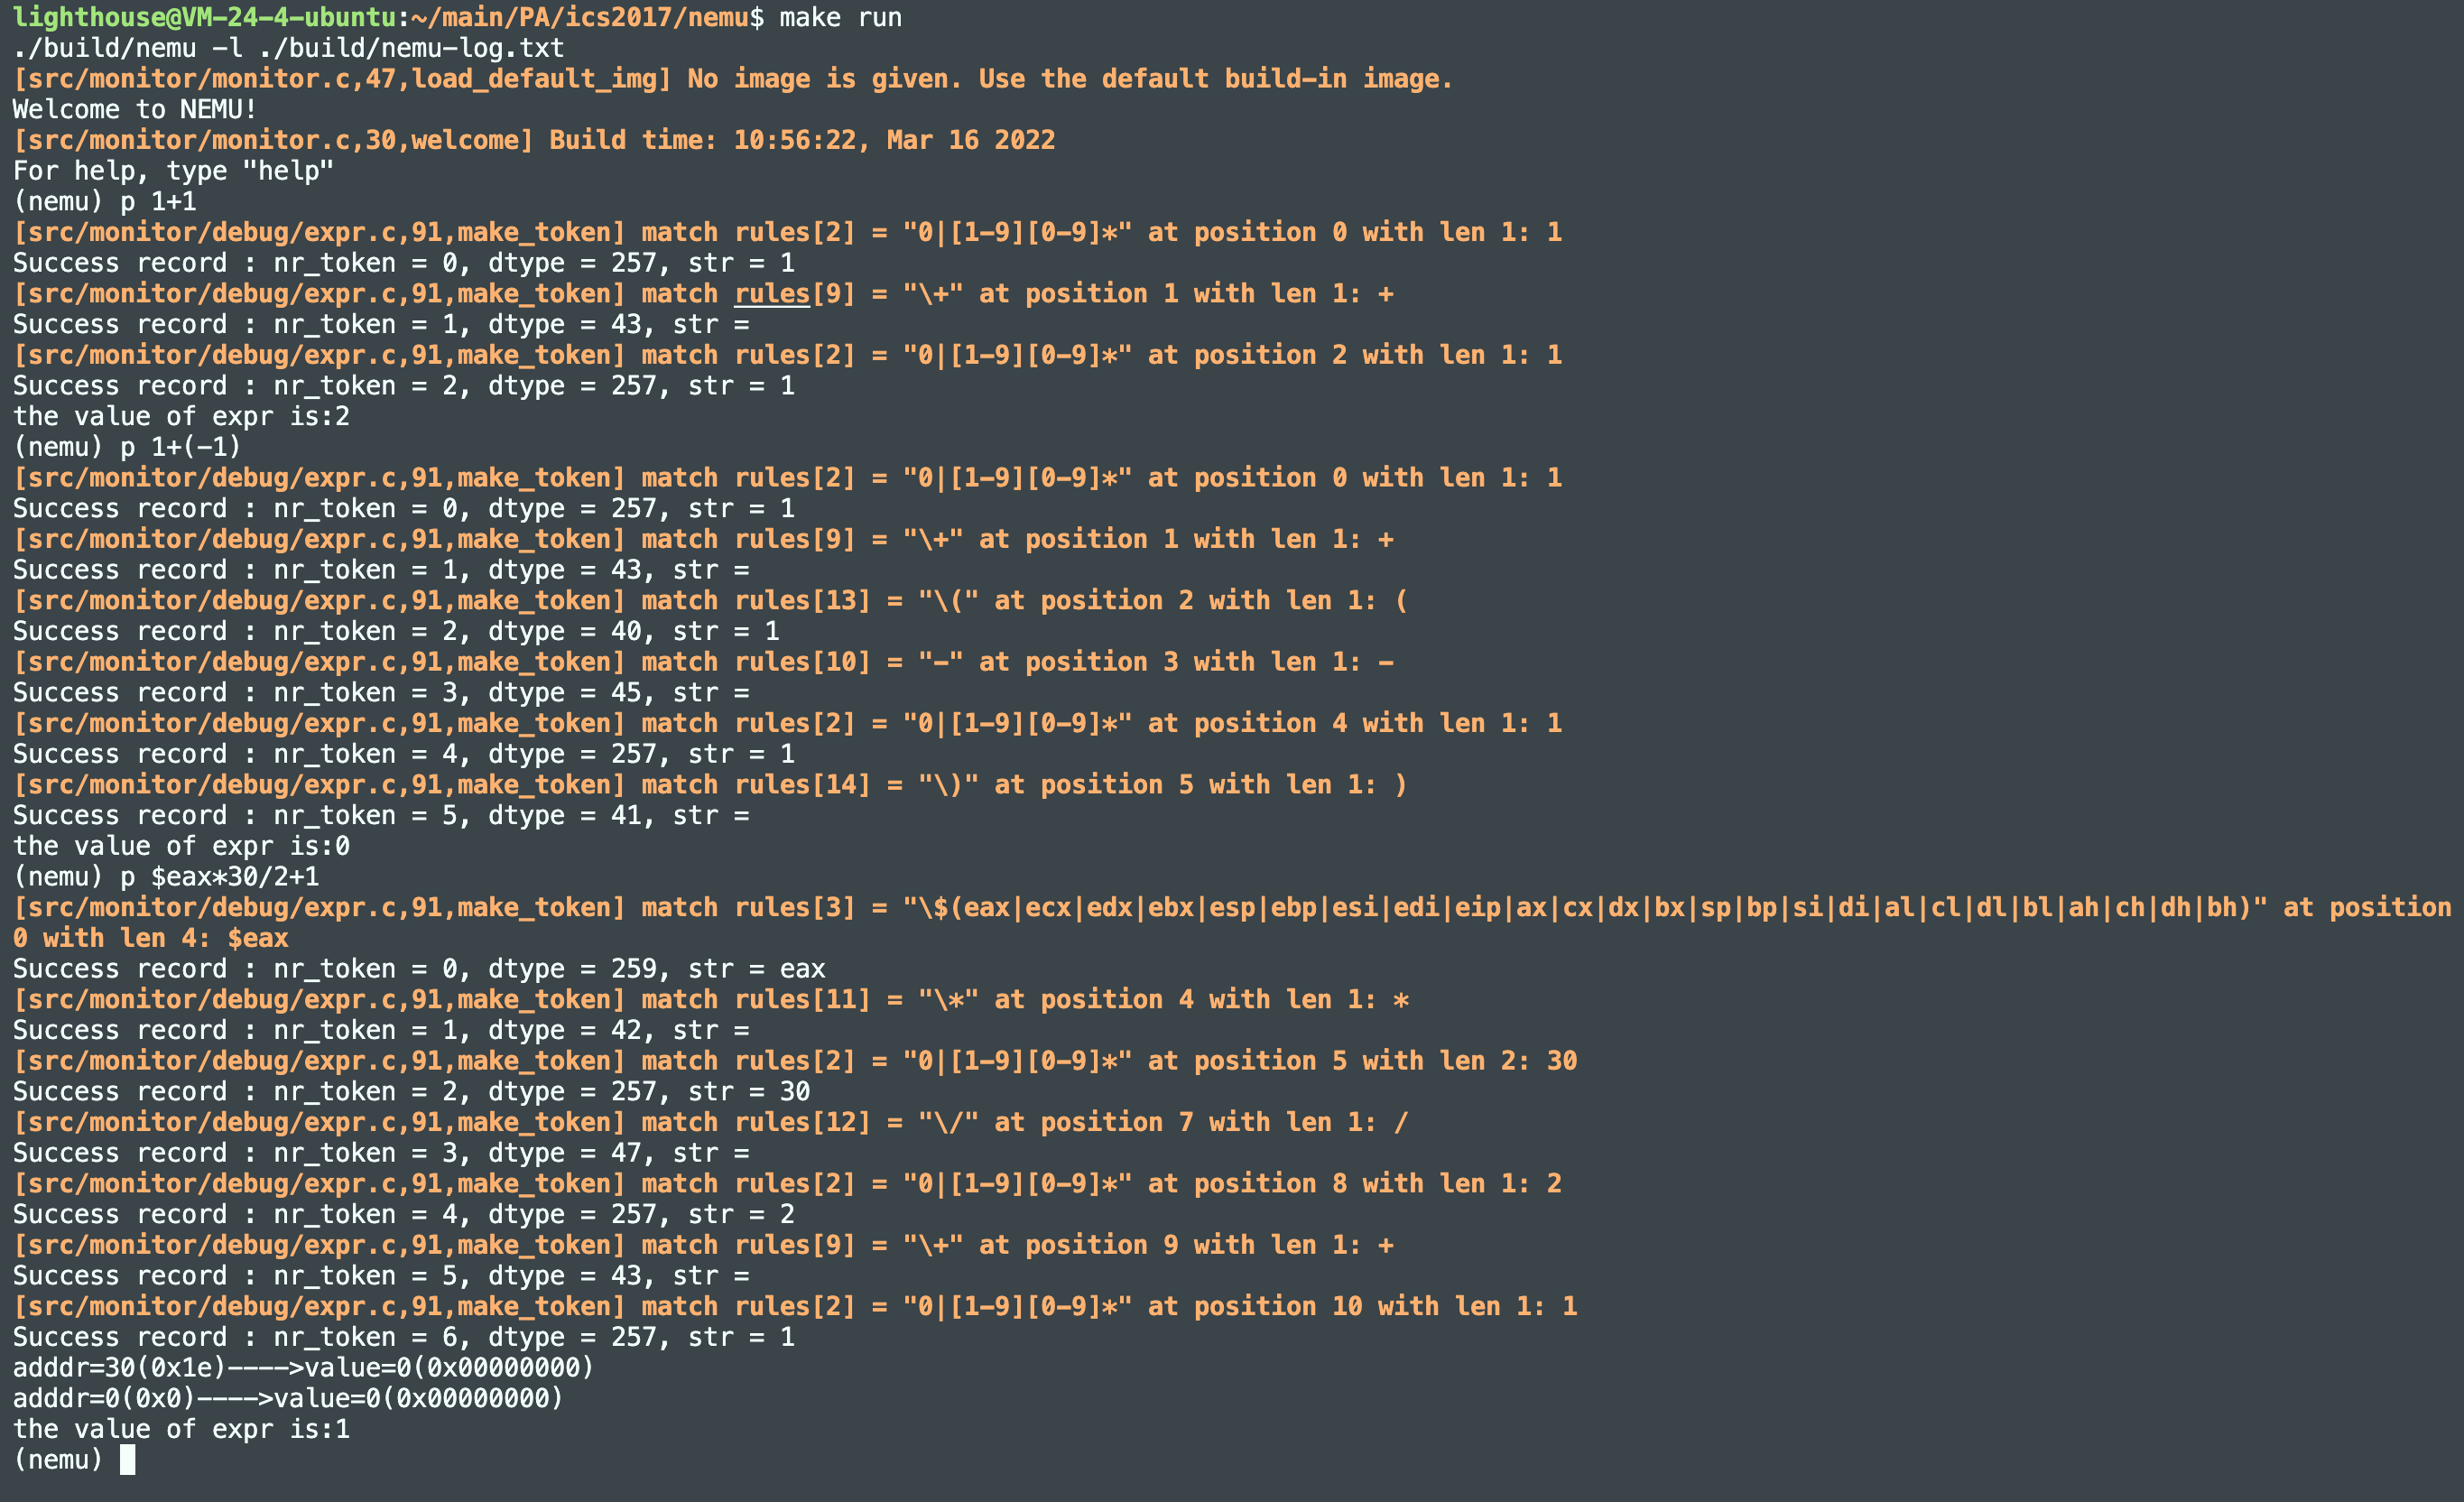
\includegraphics[scale = 0.3]{6}
  \end{center}
\end{itemize}



\section{阶段三}
\subsection*{监视点和断点}
这一部分的主要工作是通过实现两个链表(free和head)进行维护的,其代表空闲的和占用的监视点。主要工作和代码在nemu/include/ monitor/watchpoint.h和nemu/src/monitor/debug/watchpoint.c文件中实现。
\par 首先是关于实现方式的,如果删除某个监视点,其余监视点不会递补该监视点的编号(这操作实际上减少了部分工作量),新增加的监视点则会在最大的监视点编号上继续增加。监视点结构及其初始化的代码如下:
\begin{lstlisting}[language = C]
typedef struct watchpoint {
  int NO;
  struct watchpoint *next;

  /* TODO: Add more members if necessary */
  int old; //旧的值
  char e[32]; //表达式
  int hitNum; //记录触发次数

} WP;

//结构初始化
void init_wp_pool() {
  int i;
  for (i = 0; i < NR_WP; i ++) {
    wp_pool[i].NO = i;
    wp_pool[i].next = &wp_pool[i + 1];
    wp_pool[i].old = 0;
    wp_pool[i].hitNum = 0;
  }
  wp_pool[NR_WP - 1].next = NULL;

  head = NULL;
  free_ = wp_pool;
  used_next = 0;
}
\end{lstlisting}
\par 接下来,我们创建new\_up函数和free\_up函数来创建和删除监视点。主要思路是在添加监视点时,首先查找是否有足够的位置,如果有的话从链表中返回一个空闲的监视点结构,并更新head链表,将新添加的监视点添加到其尾部;在删除监视点的时候,先遍历head链表找到要被删除的监视点进行释放,然后更新free链表对空闲的监视点进行更新。其主要代码如下:
\begin{lstlisting}[language = C]
bool new_wp(char *args) {
  //从free链表中返回一个空闲监视点结构
  if(free_ == NULL) {
    assert(0);
  }
  WP* result = free_;
  free_ = free_ -> next;

  result -> NO = used_next;
  used_next++; 
  result -> next = NULL; 
  strcpy(result -> e, args);
  result -> hitNum = 0; 
  bool is_success;
  result -> old = expr(result -> e, &is_success); //计算旧的值
  if(is_success == false) {
    printf("error in new_wp; expression fault!\n");
    return false;
  }

  wptemp = head;
  if(wptemp == NULL) {
    head = result;
  }
  else {
    while (wptemp -> next != NULL)
    {
      wptemp = wptemp -> next;
    }
    wptemp -> next = result;
  }
  printf("Success: set watchpoint %d, oldvalue = %d\n", result -> NO, result -> old);
  return true;
}

//删除监视点
bool free_wp(int num) {
  WP *chosen = NULL; 
  if(head == NULL) {
    printf("no watch point now\n");
    return false;
  }
  if(head -> NO == num) {
    chosen = head;
    head = head -> next;
  }
  else {
    wptemp = head;
    while (wptemp != NULL && wptemp -> next != NULL)
    {
      /* code */
      if(wptemp -> next -> NO == num) {
        chosen = wptemp -> next;
        wptemp -> next = wptemp -> next -> next;
        break; 
      }
      wptemp = wptemp -> next;
    }
  }
  if(chosen != NULL) {
    chosen -> next = free_;
    free_ = chosen;
    return true;
  }
  return false;
}
\end{lstlisting}
\par 同时,我们还对监视点进行实时监测,其主要调用了nemu/include/cpu/exe.c中的cpu\_exec()函数。通过在cpu每执行一次命令是都检查一下所有的监视点的表达式的值是否发生了变化,如果发生了则打印变化信息来实现。其主要代码如下
\begin{lstlisting}[language = C]
void print_wp() {
  if(head == NULL) {
    printf("no watchpoint now\n");
    return;
  }
  printf("watchpoint:\n");
  printf("NO.  expr    hitTimes\n");
  wptemp = head;
  while (wptemp != NULL)
  {
    printf("%d  %s    %d\n", wptemp -> NO, wptemp -> e, wptemp -> hitNum);
    wptemp = wptemp ->next;
  }
}

bool watch_wp() {
  bool is_success;
  int result;
  if(head == NULL) {
    return true;
  } 
  wptemp = head;
  while (wptemp != NULL)
  {
    /* code */
    result = expr(wptemp -> e, &is_success);
    if(result != wptemp -> old)
    {
      wptemp -> hitNum += 1;
      printf("Hardware watchpoint %d:%s\n", wptemp -> NO, wptemp -> e);
      printf("Old value:%d\nNew valus:%d\n\n", wptemp -> old, result);
      wptemp -> old = result;
      return false;
    }
    wptemp = wptemp -> next;
  }
  return true;
}
\end{lstlisting}
\par 实验效果如下图所示
\begin{center}
  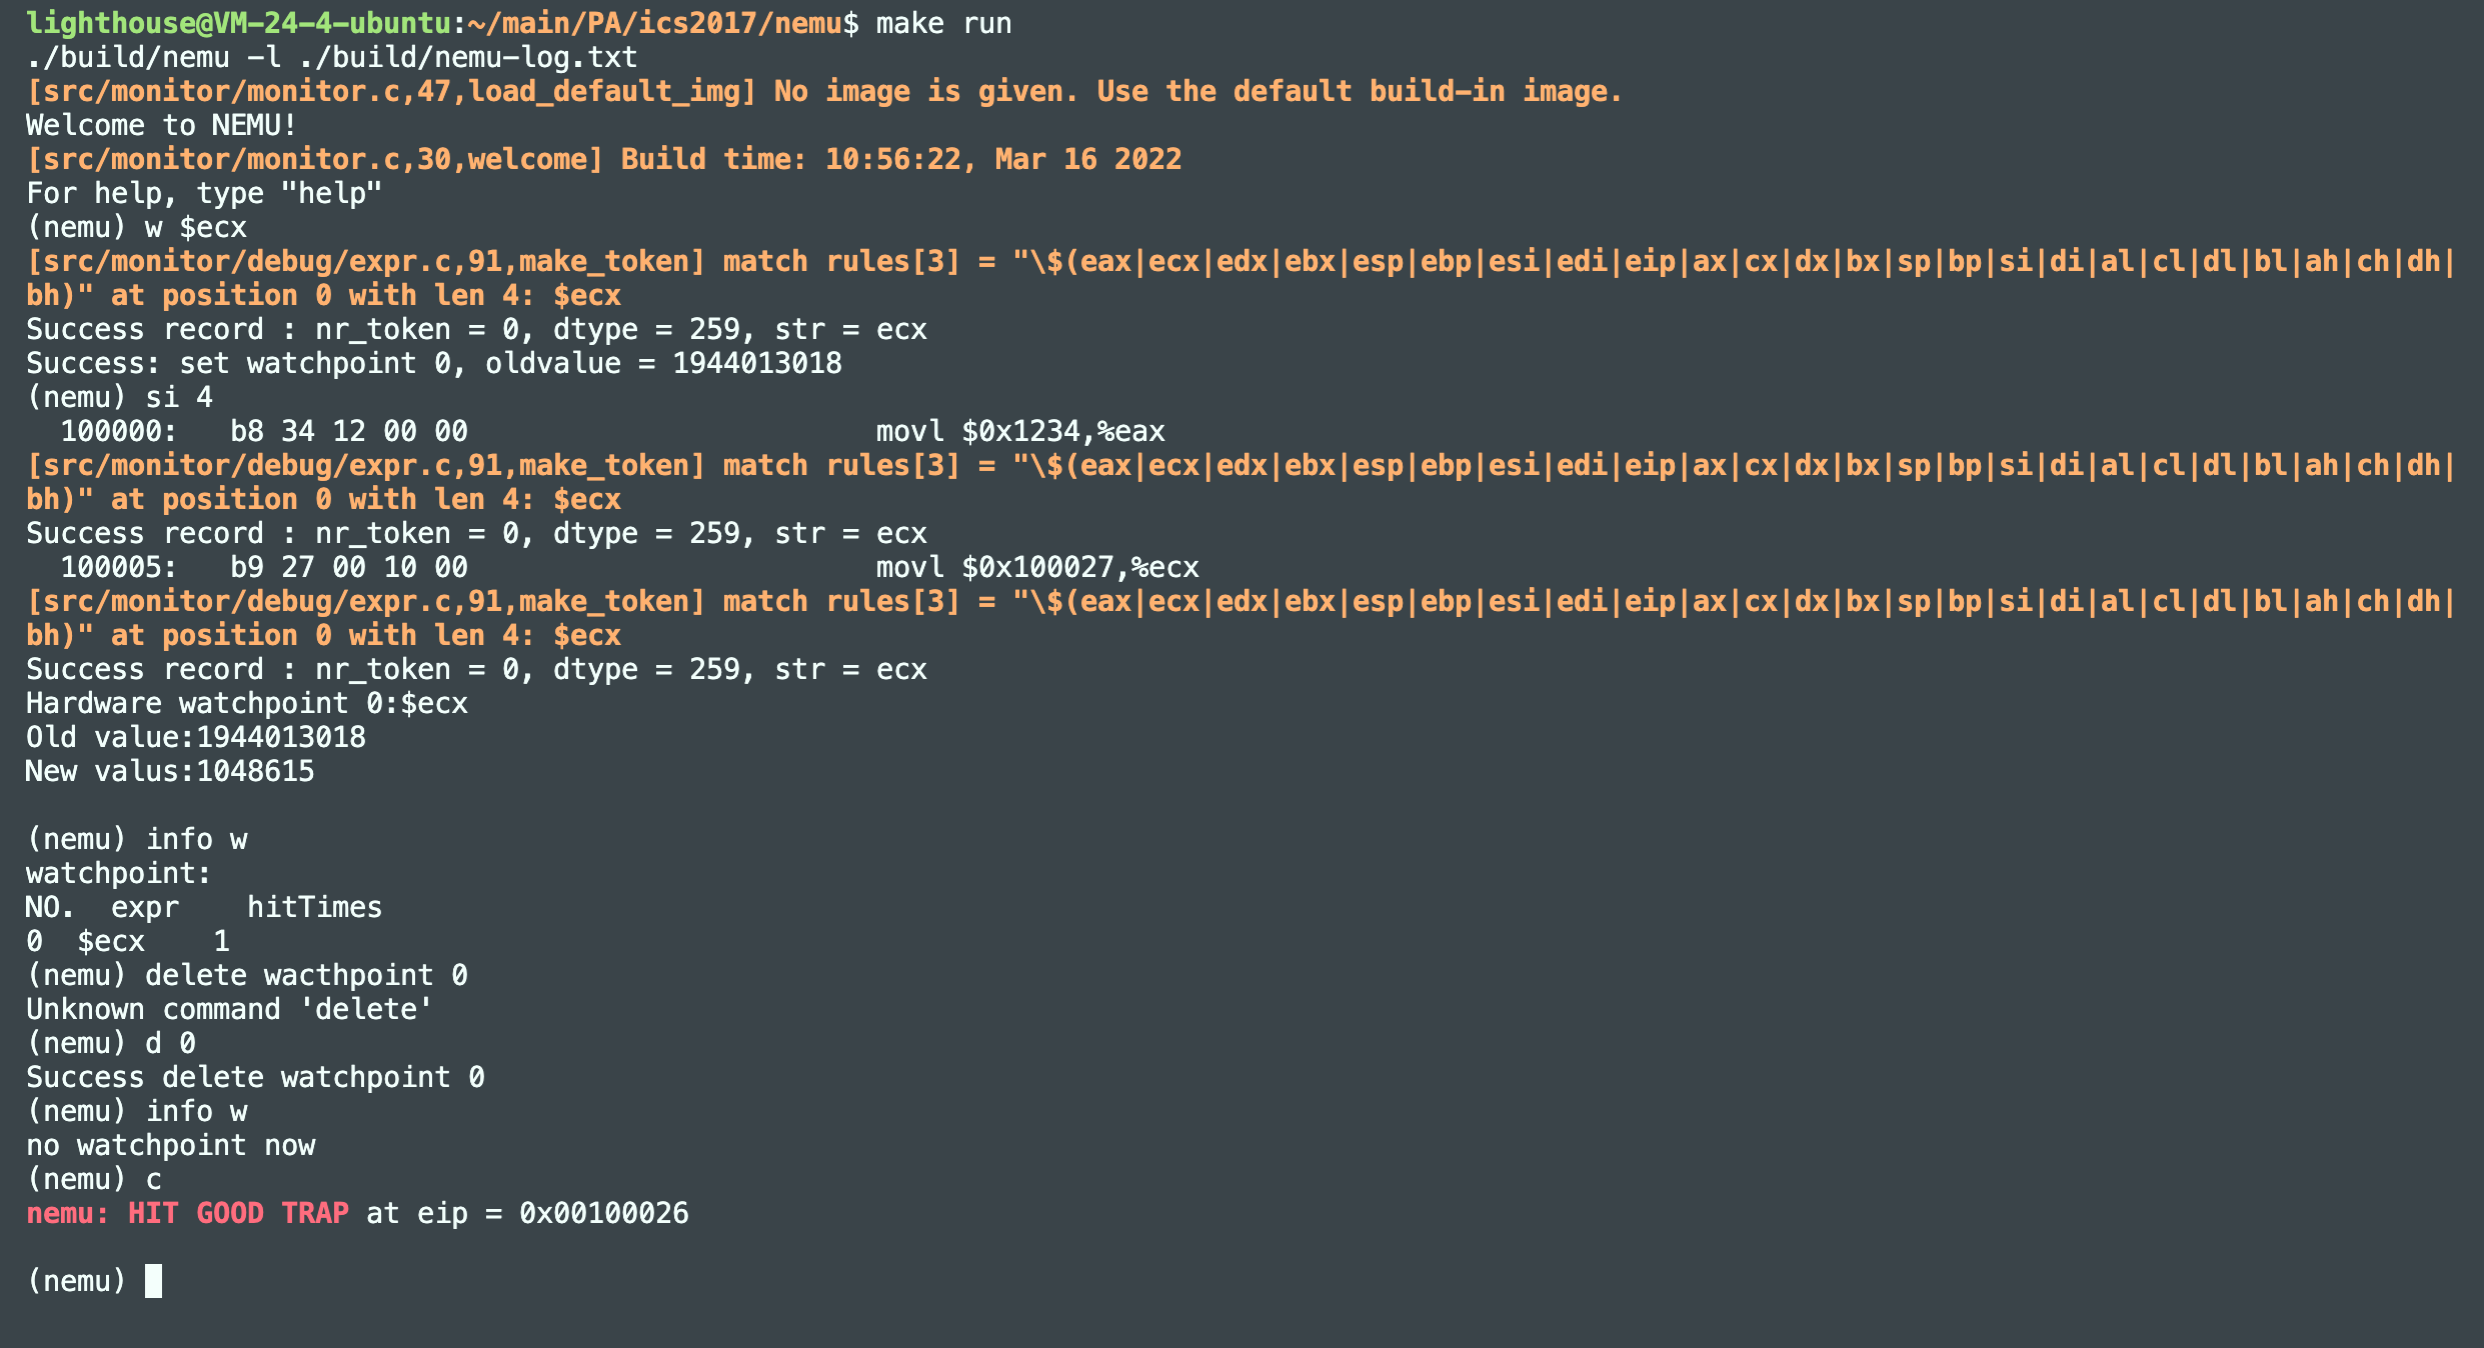
\includegraphics[scale = 0.3]{7}
\end{center}

\section{必答题}
\subsection{查阅i386手册回答问题}
\subsubsection{EFLAGS 寄存器中的 CF 位是什么意思?}
CF是Carry Flag的缩写,位于EFLAGS的第0位,是标志进位的意思。用来允许一条指令的结果影响后面的指令,即一些指令用于设置高位进位或借位,否则清0。
该结果是位于i386-2.3Register(P33)和i386-附录C(P419)
\begin{center}
  \includegraphics*[scale = 0.45]{8}
\end{center}
\subsubsection{ModR/M 字节是什么?}
ModR/M是opcode(操作码)后面的一个字节,用来表示操作数是在内存中还是在寄存器。
\subsubsection{mov 指令的具体格式是怎么样的?}
maaas



% \section{}
% \subsection{第一节}
% 如图\ref{fig:1}所示
% \begin{figure}[H]
%     \centering
%     
\includegraphics[scale=0.3]{NKU.png}
%     \caption{Caption}
%     \label{fig:1}
% \end{figure}

% 表
% \begin{table}[!htbp]
%   \centering
%   \begin{tabular}{ccccccccccc}
%   \toprule  
%   N/n$\backslash$Algo& naive-conv& naive-pool& omp-conv& omp-pool\\
%   \midrule
%   64/2& 0.0167& 0.01255& 0.04142& 0.03799\\
%   64/4& 0.03599&0.0394& 0.0458& 0.0421\\
%   \bottomrule
%   \end{tabular}
%   \caption{性能测试结果(4线程)(单位:ms)}
% \end{table}

% 带单元格表格
% \begin{table}[!htbp]
%   \centering
%   \begin{tabular}{|c|c|c|c|c|c|c|}
%   \hline
%   \multicolumn{2}{|c|}{ \multirow{2}*{$Cost$} }& \multicolumn{5}{c|}{To}\\
%   \cline{3-7}
%   \multicolumn{2}{|c|}{}&$A$&$B$&$C$&$D$&$E$\\
%   \hline
%   \multirow{3}*{From}&$B$&7&0&1&3&8\\
%   \cline{2-7}
%   &$C$&8&1&0&2&7\\
%   \cline{2-7}
%   &$D$&8&3&2&0&5\\
%   \hline
%   \end{tabular}
%   \caption{结点C距离向量表(无毒性逆转)}
% \end{table}

% %——————————————————————————————————————
% \subsection{第二节}
% 伪代码

% \begin{breakablealgorithm} 
%   \caption{初始化obj文件信息——对应MeshSimplify类中readfile函数,Face类calMatrix函数} 
%   \begin{algorithmic}[1] %每行显示行号  
%       \Require obj文件,顶点、边、面列表
%       \Ensure 是否读取成功
%       \Function {calMatrix}{$Face$}  
%               \State $normal \gets e1×e2$  
%               \State $normal \gets normal/normal.length$
%               \State $temp[] \gets {normal.x, normal.y, normal.z, normal· Face.v1}$
%               \State $Matrix[i][j]=temp[i] * temp[j]$ 
%               \State \Return{$Matrix$}  
%       \EndFunction
%       \State 根据obj的v和f区分点面信息,读取并加入列表
%       \State $scale \gets $记录点坐标中距离原点最远的分量,以便后续OpenGL进行显示
%       \State $ori \gets $记录中心点,便于OpenGL显示在中心位置,避免有的obj偏移原点较多
%       \State 根据三角面片信息,计算一个面的三条边
%       \State 计算每个面的矩阵$\gets calMatrix$
%       \State 将每个面的矩阵加到各点,由点维护\\
%       \Return True
%   \end{algorithmic}  
% \end{breakablealgorithm}

% 代码
% \begin{lstlisting}[title=逐列访问平凡算法,frame=trbl,language={C++}]
%   void ord()   
%   {
%       double head,tail,freq,head1,tail1,timess=0; // timers
%       init(N);
%       QueryPerformanceFrequency((LARGE_INTEGER *)&freq );
%       QueryPerformanceCounter((LARGE_INTEGER *)&head);
%       for (int i=0; i<NN; i++)
%           for (int j=0; j<NN; j++)
%               col_sum[i] += (b[j][i]*a[j]);
%       QueryPerformanceCounter ((LARGE_INTEGER *)& tail) ;
%       cout << "\nordCol" <<(tail-head)*1000.0 / freq<< "ms" << endl;
%   }
% \end{lstlisting}


% %——————————————————————————————————————
% \subsection{第三节}

% 参考文献\cite{adams1995hitchhiker}\cite{shin2016deep}
    
% 多行公式
% \begin{align}
%   a+b = a + b \\
%   \frac{a+b}{a-b}
% \end{align}

% 行内公式:$\sum^N_{i=1}$

% \textbf{超链接}  \href{http://youtube.com/}{YouTube}

% 带标号枚举
% \begin{enumerate}
%   \item 1
%   \item 2
% \end{enumerate}

% 不带标号枚举
% \begin{itemize}
%   \item 1
%   \item 2
% \end{itemize}

% \xiaosi{切换字体大小}

% %----------------------------------------------------------------
% \section{总结}

% %----------------------------------------------------------------
% \newpage
% \bibliographystyle{plain}
% \bibliography{references} 
\end{document}
